

\tikzset{every picture/.style={line width=0.75pt}} %set default line width to 0.75pt        

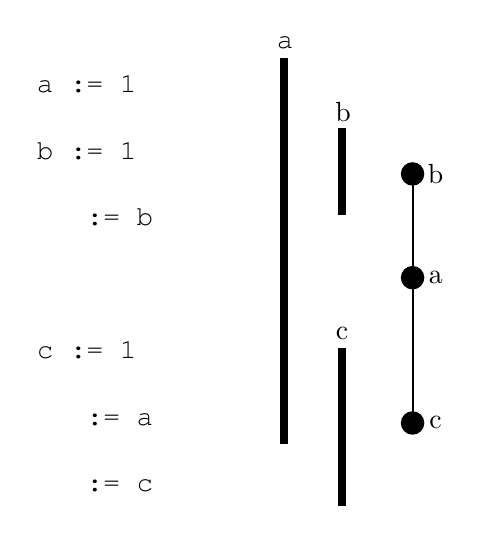
\begin{tikzpicture}[x=0.75pt,y=0.75pt,yscale=-1,xscale=1
                   ,bullet/.style={circle, fill, inner sep=3pt}]
%uncomment if require: 
%\path (0,300); %set diagram left start at 0, and has height of 300

%Shape: Boxed Line [id:dp6151775546096955] 
\draw [line width=1mm] (168, 24) -- (168,210); % a
\draw [line width=1mm] (196, 58) -- (196,100); % b
\draw [line width=1mm] (196,164) -- (196,240) ; % c

% Text Node
\draw (77,133) node  [align=left] {
{\fontfamily{pcr}\selectfont a := 1}\\\\ 
{\fontfamily{pcr}\selectfont b := 1}\\\\
{\fontfamily{pcr}\selectfont \ \ \ := b}\\\\
{\fontfamily{pcr}\selectfont }\\\\
{\fontfamily{pcr}\selectfont c := 1}\\\\
{\fontfamily{pcr}\selectfont \ \ \ := a}\\\\
{\fontfamily{pcr}\selectfont \ \ \ := c}};
% Text Node
\draw (168.57,24.88) node  [align=left] {{\fontfamily{pcr}\selectfont a}\\};
% Text Node
\draw (196.5,58) node  [align=left] {b\\};
% Text Node
%\draw (166.5,200) node  [align=left] {{\fontfamily{pcr}\selectfont a}\\};
% Text Node
%\draw (216.5,97.5) node  [align=left] {c\\};
% Text Node
%\draw (243.5,134.86) node  [align=left] {d\\};
% Text Node
\draw (196,164.86) node  [align=left] {c\\};

\draw (230, 80) node[bullet] {};
\draw (230, 80) node[align=left] {\ \ \ \ \ b};
\draw (230,130) node[bullet] {};
\draw (230,130) node[align=left] {\ \ \ \ \ a};
\draw (230,200) node[bullet] {};
\draw (230,200) node[align=left] {\ \ \ \ \ c};
\draw (230,80) -- (230,130) -- (230,200); % a
\end{tikzpicture}
